\def\year{2020}\relax
%File: formatting-instruction.tex
\documentclass[letterpaper]{article} % DO NOT CHANGE THIS
\usepackage{aaai20}  % DO NOT CHANGE THIS
\usepackage{times}  % DO NOT CHANGE THIS
\usepackage{helvet} % DO NOT CHANGE THIS
\usepackage{courier}  % DO NOT CHANGE THIS
\usepackage[hyphens]{url}  % DO NOT CHANGE THIS
\usepackage{graphicx} % DO NOT CHANGE THIS
\urlstyle{rm} % DO NOT CHANGE THIS
\def\UrlFont{\rm}  % DO NOT CHANGE THIS
\usepackage{graphicx}  % DO NOT CHANGE THIS
\frenchspacing  % DO NOT CHANGE THIS
\setlength{\pdfpagewidth}{8.5in}  % DO NOT CHANGE THIS
\setlength{\pdfpageheight}{11in}  % DO NOT CHANGE THIS

\usepackage{amsthm}
\usepackage{mathtools}
\usepackage{tikz}
\usetikzlibrary{positioning}
\usepackage{algorithm}
\usepackage{algpseudocode}
\usepackage{algorithmicx}

\DeclarePairedDelimiter\ceil{\lceil}{\rceil}
\DeclarePairedDelimiter\floor{\lfloor}{\rfloor}
\newcommand{\tup}[1]{\langle #1 \rangle}
\renewcommand{\cal}[1]{\mathcal{#1}}
\newcommand{\R}{\mathbb{R}}
\newcommand{\eps}{\varepsilon}
\newcommand{\Ch}{\mathit{Ch}}
\newcommand{\ch}{\mathit{ch}}
\newcommand{\CC}{\mathit{CC}}
\newcommand{\core}{\mathit{Core}}
\newcommand{\samples}{\omega}

\newtheorem{definition}{Definition}
\newtheorem{theorem}{Theorem}
\newtheorem{proposition}{Proposition}

\usepackage{multirow}
%\nocopyright
%PDF Info Is REQUIRED.
% For /Author, add all authors within the parentheses, separated by commas. No accents or commands.
% For /Title, add Title in Mixed Case. No accents or commands. Retain the parentheses.
 \pdfinfo{
/Title (Learning Cooperative Solution Concepts from Data)
/Author (Wei Lu, Alan Tsang, Yair Zick)
/Keywords (Game Theory)
} %Leave this	
% /Title ()
% Put your actual complete title (no codes, scripts, shortcuts, or LaTeX commands) within the parentheses in mixed case
% Leave the space between \Title and the beginning parenthesis alone
% /Author ()
% Put your actual complete list of authors (no codes, scripts, shortcuts, or LaTeX commands) within the parentheses in mixed case. 
% Each author should be only by a comma. If the name contains accents, remove them. If there are any LaTeX commands, 
% remove them. 

% DISALLOWED PACKAGES
% \usepackage{authblk} -- This package is specifically forbidden
% \usepackage{balance} -- This package is specifically forbidden
% \usepackage{caption} -- This package is specifically forbidden
% \usepackage{color (if used in text)
% \usepackage{CJK} -- This package is specifically forbidden
% \usepackage{float} -- This package is specifically forbidden
% \usepackage{flushend} -- This package is specifically forbidden
% \usepackage{fontenc} -- This package is specifically forbidden
% \usepackage{fullpage} -- This package is specifically forbidden
% \usepackage{geometry} -- This package is specifically forbidden
% \usepackage{grffile} -- This package is specifically forbidden
% \usepackage{hyperref} -- This package is specifically forbidden
% \usepackage{navigator} -- This package is specifically forbidden
% (or any other package that embeds links such as navigator or hyperref)
% \indentfirst} -- This package is specifically forbidden
% \layout} -- This package is specifically forbidden
% \multicol} -- This package is specifically forbidden
% \nameref} -- This package is specifically forbidden
% \natbib} -- This package is specifically forbidden -- use the following workaround:
% \usepackage{savetrees} -- This package is specifically forbidden
% \usepackage{setspace} -- This package is specifically forbidden
% \usepackage{stfloats} -- This package is specifically forbidden
% \usepackage{tabu} -- This package is specifically forbidden
% \usepackage{titlesec} -- This package is specifically forbidden
% \usepackage{tocbibind} -- This package is specifically forbidden
% \usepackage{ulem} -- This package is specifically forbidden
% \usepackage{wrapfig} -- This package is specifically forbidden
% DISALLOWED COMMANDS
% \nocopyright -- Your paper will not be published if you use this command
% \addtolength -- This command may not be used
% \balance -- This command may not be used
% \baselinestretch -- Your paper will not be published if you use this command
% \clearpage -- No page breaks of any kind may be used for the final version of your paper
% \columnsep -- This command may not be used
% \newpage -- No page breaks of any kind may be used for the final version of your paper
% \pagebreak -- No page breaks of any kind may be used for the final version of your paperr
% \pagestyle -- This command may not be used
% \tiny -- This is not an acceptable font size.
% \vspace{- -- No negative value may be used in proximity of a caption, figure, table, section, subsection, subsubsection, or reference
% \vskip{- -- No negative value may be used to alter spacing above or below a caption, figure, table, section, subsection, subsubsection, or reference

\setcounter{secnumdepth}{2} %May be changed to 1 or 2 if section numbers are desired.

% The file aaai20.sty is the style file for AAAI Press 
% proceedings, working notes, and technical reports.
%
\setlength\titlebox{2.5in} % If your paper contains an overfull \vbox too high warning at the beginning of the document, use this
% command to correct it. You may not alter the value below 2.5 in
\title{Learning Cooperative Solution Concepts from Data}
%Your title must be in mixed case, not sentence case. 
% That means all verbs (including short verbs like be, is, using,and go), 
% nouns, adverbs, adjectives should be capitalized, including both words in hyphenated terms, while
% articles, conjunctions, and prepositions are lower case unless they
% directly follow a colon or long dash
\author{Wei Lu,\\
School of Computing\\
National University of Singapore\\
weilu@u.nus.edu
\And
Alan Tsang,\\
School of Computing\\
National University of Singapore\\
akhtsang@nus.edu.sg
\And
Yair Zick\\
School of Computing\\
National University of Singapore\\
dcsyaz@nus.edu.sg
}

 \begin{document}

\maketitle

\begin{abstract}
Stability solution concepts have been extensively studied in the context of hedonic games. However, most past work has been purely theoretical and assumes complete visibility of all agent preferences, which is impractical in real world settings. Recent work has introduced the theory foundation of Probably Approximately Correct (PAC) stability to model stability under uncertainty through sampling. In this paper, we propose an algorithmic improvement for discovering PAC stable solutions. We apply the improved algorithm on Knesset voting data and discover that the PAC stable solutions reflect Knesset members' political positions at large, and are able to reveal a few politicians whose voting behavior breaks their party lines. We also demonstrate empirically that this PAC hedonic game modeling approach compares favorably to clustering approach.
\end{abstract}

\noindent Introduction TODO

\section{Preliminaries}

\subsection{Hedonic Games}
Hedonic games are a sub-class of nontransferable utility cooperative games. A hedonic game is a coalition formation game with hedonic preferences. A coalition formation game aims to divide the set of all players $N$ into disjoint coalitions, formally known as a coalition structure, often denoted as $\pi$. Hedonic preference means that every player only cares about the coalition they belong to, which implies that the inter-coalitional dependencies are completely ignored. The description of a hedonic game could be exponentially large in the number of players, as each player needs to rank all possible coalitions they may belong to.

\begin{definition}
  A {\it hedonic game} is a pair $(N, P)$, where $N$ is a finite set of players $1, \cdots, n$ and $P$ is a {\it preference profile} consisting of preference relations $\succeq_i$ for every player $i \in N$: $P = (\succeq_1, \cdots, \succeq_n)$. A {\it preference relation} $\succeq_i$ is a reflective, complete, and transitive binary relation on $mathcal{N}_i$, where $mathcal{N}_i$ is the set of all non-empty subset of $N$ that includes player $i$: $mathcal{N}_i \{S \subseteq N: i \in S, S \neq \emptyset \}$
\end{definition}

\subsection{Top Responsive Games}
The intuition behind top responsiveness is that every player derives their utility from the most preferred subset players of the coalition they belong. If two coalitions, with one containing the other, yield the same utility for a player, the tie is broken in favor of the smaller coalition. Formally, for a game to satisfy {\it top responsiveness}, it requires the following three conditions to hold true for any player $i \in N$, and any coalition that may contain player $i$: $S, T \in \mathcal{N}_i$:
\begin{enumerate}
  \item $|Ch(i, S)| = 1$.
  \item if $ch(i, S) \succ_i ch(i, T)$ then $S \succ_i T$
  \item if $ch(i, S) = ch(i, T)$ and $S \subset T$ then $S \succ_i T$
\end{enumerate}

Where $Ch(i, S)$ denotes the choice sets of player $i$ in coalition $S$, formally defined as:

$Ch(i, S) = \{S' \subseteq S: (i \in S') \wedge (S' \succeq_i S'' \forall S'' \subseteq S)\}$

The unique choice set in $Ch(i, S)$ is denoted as $ch(i, S)$.

\subsection{Appreciation of Friends Preference Profile}

In this preference model, a player classifies other players as either friends or enemies, and prefers any coalition with more friends and fewer enemies:

\begin{definition}
  Let $G_i$ be player $i$'s set of friends, and $B_i$ the set of enemies. $G_i \cup B_i \cup i = N$ and $G_i \cap B_i = \emptyset$. A preference profile $P^f$ is based on {\it appreciation of friends} if for all player $i \in N$, $S \succeq_i T$ if and only if

\begin{enumerate}
  \item $|S \cap G_i| > |T \cap G_i|$ or
  \item $|S \cap G_i| = |T \cap G_i|$ and $|S \cap B_i| \leq |T \cap B_i|$
\end{enumerate}
\end{definition}

\cite{SuSu10} have shown that the domain of preference profiles based on appreciation of friends is a proper subdomain of top responsive preference profiles. Some top responsive games do not satisfy the requirements of appreciation of friends, for example, $N = \{1, 2, 3\}$, preference relation $\{1, 2\} \succ_1 \{1, 2, 3\} \succ_1 \{1, 3\}$ satisifies top responsiveness but not apprciation of friends.

\subsection{Mutuality}
Mutaulity in the context of top responsive games means that for all $i, j \in N$, for all coalition that contains $i$ and $j$: $S \in \mathcal{N}_i \cap \mathcal{N}_j$, $i \in ch(j, S)$ if and only if $j \in ch(i, S)$. Mutuality provides guarantees for solutions that satisfy stronger notion of stability, which we will discuss after the stability concepts defitions.

\subsection{Stability Concepts}
Core stable and strictly core stable are solution concepts useful for modeling real world scenarios because they represent a stable state where no subset of players can be better off by deviating from. A hedonic game solution $\pi$ is core stable when there is no strongly blocking coalition. A coalition $S \subseteq N$ strongly blocks a coalition structure $\pi$ if every player $i \in S$ strictly prefers $S$ over its current coalition $\pi(i)$. Similarly, a hedonic game is strictly core stable when there is no weakly blocking coalition. A coalition $S \subseteq N$ weakly blocks a coalition structure $\pi$ if every player $i \in S$ weakly prefers $S$ over its current coalition $\pi(i)$ and there exists at least one player $j \in S$ who strictly prefers $S$ over $\pi(j)$.

Strong Nash Stability (SNS) and Strict Strong Nash Stability (SSNS) is a pair of stronger stable concepts compared to Core (C) and Strict Core (SC) stabilities, that are also based on group deviations. If a partition $\pi' \neq \pi$ exists with movement of players $S \subseteq N$ and $S \neq \emptyset$ (denoted as $\pi \xrightarrow{S} \pi'$), where $\forall i \in S$, $\pi'(i) \succ_i \pi(i)$, and $\forall j \in N\text{\textbackslash}S$, $\pi'(j) = \pi(j)$, then $S$ strongly Nash blocks $\pi$. A partition that admits no strongly Nash blocking set $S \subseteq N$ is said to be strong Nash stable. A non-empty set of player $S \subseteq N$ weakly Nash blocks $\pi$ if $\forall i \in S$, $\pi'(i) \succeq_i \pi(i)$ and $\exists j \in S$, $\pi'(j) \succ_j \pi(j)$. A partition that admits no weakly Nash blocking set $S \subseteq N$ is said to be strict strong Nash stable.

Nash stable is the strongest stability notion based on individual deviations, as it doesn't account for the disutility of the group an individual player is joining or leaving. A partition is Nash stable if no player can benefit by moving unilaterally to another coalition.

TODO: Example of Core that's not SNS, example of SNS that's not strict core

\begin{figure}
\centering
\begin{tikzpicture}[
squarednode/.style={rectangle, draw=white!60, fill=white!5, very thick, minimum size=5mm},
]
%Nodes
\node[squarednode]      (SSNS)                             {SSNS};
\node[squarednode]      (SNS)       [below left=of SSNS]   {SNS};
\node[squarednode]      (NS)        [below=of SNS]         {NS};
\node[squarednode]      (SC)        [below right=of SSNS]  {SC};
\node[squarednode]      (C)         [below=of SC]          {C};

%Lines
\draw[->] (SSNS.south west) -- (SNS.north east);
\draw[->] (SNS.south) -- (NS.north);
\draw[->] (SSNS.south east) -- (SC.north west);
\draw[->] (SC.south) -- (C.north);
\draw[->] (SNS.south east) -- (C.north west);
\end{tikzpicture}
\caption{Relationships between stability concepts for hedonic games: Strict strong Nash stable implies strict core and strong Nash stable. Strong Nash stable immplies core and Nash stable. Strict core implies core.}
\end{figure}

\subsection{Complete Preference Profile Algorithms} \label{section:top_covering}

\cite{ALCALDE2004869} showed that top responsive games guarantee the existence of a core stable partition, which is discoverable through the Top Covering Algorithm. \cite{DIMITROV2007130} simplified the original Top Covering Algorithm and proved that it not only constructs a core, but a strict core. \cite{Dimitrov2006TopRA} also showed that adding the mutuality condition the simplified top covering algorithm produces a Nash stable partition. \cite{Aziz:2012:ESH:2343776.2343806} further proved that with mutuality the partition produced is in fact strict strong Nash stable for any top responsive game.

\begin{algorithm}[htb]
  \caption{Top Covering Algorithm}
  \label{alg:top_covering}
  \textbf{Input:} A hedonic game satisfying top responsiveness.

  \begin{algorithmic}[1]
  \State $R^1 \leftarrow N$; $\pi \leftarrow \emptyset$.

  \For{$k=1$ to $|N|$}
    \State \label{top_cover:select} Select $S^k$
    \State \label{top_cover:remove} $\pi \leftarrow \pi \cup \lbrace S^k \rbrace$ and $R^{k+1} \leftarrow  R^k \setminus S^k$
    \If {$R^{k+1} = \emptyset$}
      \State \Return $\pi$
    \EndIf
  \EndFor

  \State \Return $\pi$
 \end{algorithmic}
\end{algorithm}

Step~\ref{top_cover:select} effectively selects the smallest ``connected component'' ($CC$) in the graph induced by the remaining players as nodes and their choice sets as edges. The set of vertices of the smallest $CC$ is assigned to $S^k$. Formally, select $i\in R^k$ such that $|CC(i,R^k)| \leq |CC(j,R^k)|$ for each $j\in R^k$; and $S^k\leftarrow CC(i,R^k)$, where $CC(i, S)$ denotes the connected component with $i$ as the root node, in the graph induced by $S$ as vertices and directed edges $E$, $(i, j) \in E$ if $j \in ch(i, S)$ for all $j \in S$.

Note that the input of the top covering algorithm is the entire preference profile of all players, which is in the order of $O(2^{|N|})$. Finding the choice set for every player after each round of player removal at Step~\ref{top_cover:remove} requires scanning through every remaining player's preference relation, which makes the most expensive part of this algorithm, so this algorithm is exponential time in the number of players.

\cite{Dimitrov2006} showed that given a preference profile based on appreciation of friends $P^f$, a strictly core stable coalition structure can be found in polynomialtime in the number of players. Their algorithm effectively replaces Step~\ref{top_cover:select} of Algorithm~\ref{alg:top_covering} with finding the largest strongly connected component (SCC) in the graph induced by $R^k$. Due to the the appreciation of friends preference profile, Step~\ref{top_cover:remove} no longer requires scanning through every remaining player's preference relation for removed players, making the partition equivalently a strong decomposition of the graph induced by $N$. TODO: known algorithm complexity

\subsection{PAC Learning and PAC Stability}
Probably Approximately Correct (PAC) learning is the canonical framework aimed at providing good probabilistic approximation to functions with polynormial number of samples. A good probabilistic approximation means that with high probability of at least $1 - \delta$, the selected function has low generalization error $\varepsilon$, where $0 < \varepsilon, \delta < 1$. A hypothesis class is efficiently PAC learnable if such a good probabilistic approximation can be produced by some algorithm that has both running time and input sample size be polynormial in $n$, $\frac{1}{\varepsilon}$, and $\log{\frac{1}{\delta}}$.

In the context of hedonic games, based on a similar notion \cite{ijcai2017-380} defined that a class of hedonic games is PAC stablizable if there exists a polynormial time and input size algorithm in $n$, $\frac{1}{\varepsilon}$, and $\log{\frac{1}{\delta}}$ that produces a partition $\pi$ such that $\Pr_{S\sim D}[\text{S core blocks } \pi] < \varepsilon$. In the same paper, \cite{ijcai2017-380} also showed that top responsive games are efficiently PAC stablizable despite not PAC learnable. The PAC stable partition can be computed with Algorithm~\ref{alg:pac_top_covering}.

\begin{algorithm}[htb]
  \caption{PAC Top Covering Algorithm}
  \label{alg:pac_top_covering}
  \textbf{Input:} $\eps$, $\delta$, set $\cal S$ of $m = (2n^4 + 2n^3)\ceil{\frac{1}{\eps}\log\frac{2n^3}{\delta}}$ samples from $\cal D$
  \begin{algorithmic}[1]

  \State $R^1 \gets N$, $\pi \gets \emptyset$
  \State $\samples \gets \ceil{2n^2 \frac{1}{\eps}\log\frac{2n^3}{\delta}}$
  \For{$k=1$ to $|N|$}

    \State $\cal S' \gets$ take and remove $\samples$ samples from $\cal S$
    \State $\cal S' \gets \{T: T \in \cal S', T \subseteq R^k\}$
    \For{$i \in R^k$}
      \If{$i \notin \bigcup_{X \in \cal S'} X$}
        \State$B_{i,k} \gets \{i\}$
      \Else
        \State $B_{i,k} \in \arg\max_{T \in \cal S'}{v_i(T)}$
        \State $B_{i,k} \gets \underset{\{T \in \cal S' : \ch(i,T) = \ch(i,B_{i,k})\}}{\bigcap} T$.
      \EndIf
    \EndFor

    \For{$j = 1,\dots,|R^k|$}
      \State $\cal S'' \gets$ take and remove $\samples$ samples from $\cal S$
      \State $\cal S'' \gets \{T: T \in \cal S'', T \subseteq R^k\}$
      \For{$i \in R^k$}
        \State $B_{i,k} \gets B_{i,k} \cap \underset{T \in \cal S'' : \ch(i,T) = \ch(i,B_{i,k})}{\bigcap} T$.
      \EndFor
    \EndFor

    \State Select $i\in R^k$ such that $|CC(i,R^k)| \leq |CC(j,R^k)|$ for each $j\in R^k$.
    \State $S^k\leftarrow  CC(i,R^k)$; $\pi \leftarrow  \pi \cup \lbrace S^k \rbrace$;  and $R^{k+1} \leftarrow  R^k \setminus S^k$
    \If {$R^{k+1} = \emptyset$}
      \State \Return $\pi$
    \EndIf
  \EndFor

  \State \Return $\pi$
 \end{algorithmic}
\end{algorithm}

Where every sample $j$ consists of a coalition $S_j \subseteq N$, and the values assigned to $S_j$ by each of its member $\vec{v}(S_j) = (v_i(S_j))_{i \in S_j}$.

\section{Improvemented PAC Top Covering Algorithm}
We discovered that the PAC top covering algorithm can be made more efficient by replacing the step of finding the smallest $CC$ with finding the largest Strongly Connected Component ($SCC$). Since the PAC top covering algorithm is based on the top covering algorithm, we will show that the partition generated from finding and deleting the SCC is strictly core stable for the original top covering algorithm. Then we will analyse the running time complexity implication for the PAC version of the algorithm.

\begin{theorem}
  The modified top covering algorithm produces a strictly core stable partition given a top responsive preference profile
\end{theorem}

\begin{proof}
Assuming the resulting partition of the $SCC$ procedure $\pi$ is not strictly core stable, then there exists at least one weakly blocking coalition $S \subseteq N$ and at least one player $i \in S$ prefers S over $\pi(i)$. Consider the step when the coalition $\pi(i)$ is generated – it was the largest strongly connected component in the directed graph induced by remaining players' choice sets. In order to form $S$ which is different from $\pi(i)$, either or both of the following steps must be carried out:

\begin{enumerate}
  \item at least one player $j \in \pi(i)$ needs to be removed from $\pi(i)$
  \item at least one player $k \notin \pi(i)$ needs to be added to $\pi(i)$
\end{enumerate}

When only Step 1 is carried out, since $\pi(i)$ is a strongly connected component, $j$ has at least one incoming edge, which means it's in the choice set of at least one other player $j' \in \pi(i)$, therefore its removal makes player $j' \in S$ worse off, therefore $S$ cannot be weakly blocking $\pi$.

When only Step 2 is carried out, since player $k$ wasn't part of the strongly connected component that induces $\pi(i)$, $k$ only has incoming or outgoing edges between itself and the $SCC$ but not both types. If $k$ only has outgoing edges to $SCC$ it means adding $k$ to $\pi(i)$ will only make $k$ better off, but other players in $\pi(i)$ worse off because $S = \pi(i) \cup \{k\}$ is bigger in size $|S| > |\pi(i)$ while for any player $i' \in S, i' \neq k$ their choice set remains the same, therefore making $S$ less preferable than $\pi(i)$ for player $i' \in S, i' \neq k$ per definition of top responsiveness. Therefore $S$ is not blocking $\pi$ when $k$ only has outgoing edges to $SCC$. In the case $k$ only has incoming edges from $SCC$, it means adding $k$ to $\pi(i)$ will only make some player $i \in \pi(i)$ better off as $k$ is in their choice set. However $k$ will be made worse off by this move, since none of the player in $\pi(i)$ is in $k$'s choice set. As such, $S$ is not blocking $\pi$ when only Step 2 is carried out.

When both Step 1 and Step 2 are carried out to form $S$ from $\pi(i)$, since Step 1 is bound to make some player $j' \in \pi(i)$ worse off, the only way to compensate $j'$ is by adding someone from their choice set to $\pi(i)$. Assuming $k$ is in $j'$'s choice set, then $k$ only has incoming edges from the $SCC$, which means $k$ will be worse off by joining $\pi(i)$, so $S$ cannot be blocking $\pi$.
\end{proof}

The largest $SCC$ procedure provides a running time improvement over the smallest $CC$ procedure because finding the smallest $CC$ requires $O(V(V + E))$ time while the largest $SCC$ can be found using Tarjan's algorithm in linear time $O(V + E)$\cite{Tarjan72depthfirst}. This running time improvement is only meaningful for the PAC verison of the top covering algorithm due to the input size of the original top covering algorithm being exponential in the number of players. In addition, taking out more players in the earlier iterations also reduces the amount of computation required for the later iterations, making our experiments run much faster than what it would have been with the original $CC$ procedure.

\section{Data}
Knesset is the national legislative branch of the Israeli government. Knesset website provides data access through Open Data Protocol (OData) on all its parliament members, laws, and every member's votes on every law. We limit our dataset to the 20th Knesset (2015-2019), which is the last Knesset preseeding the current one. We downloaded all 147 parliament members' information including id, name, faction id, faction name and their votes for all 7515 bills deliberated. A vote can take on one of the following values 0 (vote canceled), 1 (vote for), 2 (vote against), 3 (abstained), 4 (did not attend). We programmatically transformed the downloaded data into comma separated values (CSV), with each row representing a bill and each column representing a parliament member, so a cell value corresponds to the vote of a given parliament member for a given bill.

\subsection{Data Preprocessing}
During data processing, we noticed that more than half of all the vote values are missing despite the presence of value 4 for ``did not attend''. It raises questions regarding the data quality. We discovered another API endpoint which provides summary information for every bill, including total number of for votes, against votes, abstained votes, and if the bill is accepted. We downloaded bill summary data set for the 20th Knesset and used it to check against the tallied vote numbers from the individual vote data. We ended up discovering more inconsistencies:

\begin{itemize}
  \item Total bills checked: 7513,
  \item Missing bills in the summary dataset: 2,
  \item Number of bills with pass/reject status inconsistent: 26,
  \item Number of bills with for count inconsistent : 273,
  \item Number of bills with against count inconsistent : 402,
  \item Number of bills with abstain count inconsistent : 2
\end{itemize}

We reached out to Knesset regarding the data inconsistency between two API endpoints, as well as the missing value issue. The Knesset data management team stated that the inconsistency is likely a result of manual vote entries instead of votes recorded as a result of pressing the electronic button. Such manual vote entries are captured by the bill summary data set but not individual member's vote data set.

For the purpose of our research, we treat the data with individual member's votes on every bill as the ground truth since it has the level of granularity required for modeling. We removed the 26 bills whose pass/reject status is inconsistent between the summary and invidual data sets, since it's most likely that the individual data is wrong.

\section{Experiments}

\subsection{Top Responsive Game Model}
Top responsiveness models a preference profile where every player derives their utility for a given coalition from the most preferred subset players in their coalition. In the context of legislature, it captures that politicians care about whose votes they stand with – they want to vote with other politicians they like. Since we do not observe quantifiable preferences of each Knesset member over other members, we will be deriving their preferences from the Knesset voting data assuming top responsiveness and mutuality. Top responsiveness guarantees a strictly core stable partition. With the addition of mutality, as discussed in \ref{section:top_covering}, a strict strong Nash stable partition can be computed using Algorithm ~\ref{alg:top_covering} if the full preference profile is given. When the complete preference profile is not available, we can use Algorithm ~\ref{alg:pac_top_covering} to approximate a strict strong Nash stable partition. We then compare the resulting partitions to party affiliations to assess the quality of our models.

\subsection{Handcrafted Value Function}
For each bill there are two natural coalitions: one formed by parliament members who voted ``for'', and the other formed by parliament members who voted ``against''. Note that the values assigned by members to their respective coalitions are not immediately well defined, so we define the player $i$'s value function for coalition $S$ as below:

\[
  v_i(S) = 
  \begin{dcases}
      1 + \frac{1}{|S|} + \frac{|S_p|}{|N|},& \text{if S is the winning majority}\\
      0,              & \text{otherwise}
  \end{dcases}
\]

$S$ can take on one of the two values $\{S_f, S_a\}$, where $S_f$ is the set of members who voted ``for'' and $S_a$ is the set of members who voted ``against''. $S_p$ denotes the set of parliament members who participated $S_p = S_f \cup S_a$. $S_f$ is the winning majority if $|S_f| > |S_a|$, vice versa. When $|S_f| = |S_a|$, $S_a$ is considered to be the winning majority.

The conditional value function captures that a winning coalition, being successfully passing a bill or successfully blocking a bill, is always worth more than a losing coalition. $\frac{1}{|S|}$ reflects that a win is considered more valuable when it's achieved with fewer members, which is also conceptually consistent with top responsive game's preference for smaller coalitions. The partition term $\frac{|S_p|}{|N|}$ gives a win more value when more parliament members voted for or against the bill. For simplicity, we assume every member in a given coalition assigns equal value to their coalition.

This handcrafted value function allows us to construct a partial preference relation for every parliment member. We programmatically verified that this partial preference profile in fact does not satisfy top responsiveness. It makes this approach analogous to improper learning.

To simulate i.i.d, we sample $\frac{3}{4}$ of the bills with replacement. We repeated the algorithm run 50 times and observed that the resulting partition is consistent with little variability. It is not core stable with respect to the partial preference profile. This is unsurprising due to the PAC model. The partition has one large coalition consisting of around 60 members and the rest are all singleton coalitions. All members of the only large coalition are from right wing parties. The singleton coalitions are likely a result of the limited size of the derived partial preference profile - Upon discovery of the smallest $CC$ in each iteration, we also remove any coalition that contains any of the removed player from the remaining player's preference relation. Since we took away a large number of players in one of the first few iterations, many coalitions are removed from remaining players' preference relations, resulting in isolated nodes in the updated graph which leads to singleton coalitions. Despite the number of singleton coalitions, the largest coalition does reflect political position of about 40\% of the parliment members.

\begin{figure}[htb]
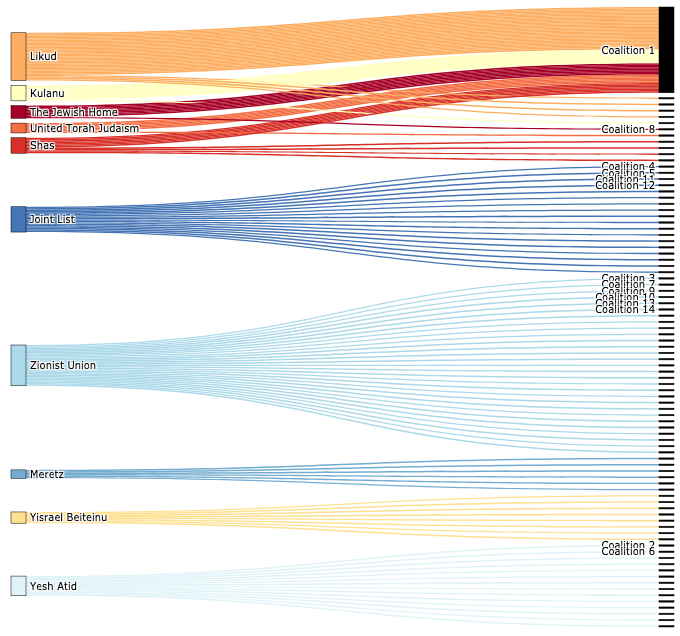
\includegraphics[width=\columnwidth]{pac_value_function}
\caption{Coalitions formed by the PAC model with the handcrafted value function, compared to party affiliations. Left wing parties are colored with blue hues, right wing red hues, center yellow hues.}
\end{figure}

\subsection{Appreciation of Friends}
Another set of experiments are based on the appreciation of friends model, which is a proper subset of top responsive games. We define friends of a player's as anyone whose votes agreed with the given player's more than disagreed. Agreed votes are only counted if the given player voted ``for'' or ``against''. We experimented with two different ways of counting the disagreed votes:

\begin{enumerate}
  \item Narrow disagreement: the other player's vote is different from mine, and is either ``for'' or ``against''
  \item Broad disagreement (selective friends): the other player's vote is different from mine
\end{enumerate}

Compared to narrow disagreement, broad disagreement leads to every player being more selective of friends. For any player, those who are not friends are considered enemies.

Note that as soon as the sets of friends and enemies are derived for each parliment member, we can expand them into a complete preference profile, and apply top covering algorithm to obtain a strict strong Nash stable partition with respect to the given preference profile. The broad disagreement setup produced a partition with 18 coalitions out of which there are two large coalitions with 66 and 58 members each. One of these two large coalitions is made of left wing party politicians, while the other of right wing party members. Together, over 84\% of the parliment members' political positions are revealed by this model. In contrast, by being slightly less selective of friends, the narrow disagreement setup resulted in the grand coalition as the strict strong Nash stable outcome. This shows that the appreciation of friends model is very sensitive to the definition of friends.

\begin{table}[h!]
\centering
\begin{tabular}{c|c|c}
\hline
Model & No. Coalitions & Norm Info Dist \\
\hline
Friends & 1 & 1 \\
Selective friends & 18 & 0.605 \\
\hline
\end{tabular}
\caption{Partitions generated using top covering algorithm, with full preference profile derived from appreciation-of-friends preference model. Friends corresponds to narrow disagreement definition model, selective friends corresponds to broad disagreement definition model}
\label{table:friends_models}
\end{table}

We then integrated the appreciation-of-friends preference profile with the PAC top covering algorithm. Similar to the value function experiment, in each iteration, we repeated sample $\frac{3}{4}$ of all the bills and use them to find every remaining player's most preferred coalition, which is used as an approximation of their choice set. With the approximated choice sets, we construct the directed graph, find the largest strongly connected component, assign all players corresponding to the vertices of the strongly connected component to a coalition as part of the final partition, remove the assigned players from the game and repeat the iteration for the remaining players.

Recall in the value function preference model, the value of any coalition is only calculated once; as we remove players, any coalitions containing any removed players are simply removed from remaining players' preference relations. For any ``for'' or ``against'' coalition of a given bill, it doesn't make sense to modify it because the value function is defined for the observed coalition based on a combination of the voting outcome and participation. In contrast, with the friends preference model, we define coalition for a given player and a sample bill as the set of players who voted the same as the given player (either ``for'' or ``against'' the bill) and we allow this coalition to shrink as players are removed from the game in each iteration of the algorithm. Therefore we need to re-evaluate every coalition for a given player and sample bill pair as removing players will change the friend count and/or the enemy count for each coalition. This makes this model more computationally expensive than the value function model.

We ran the algorithm 50 times each for the two disagreement definitions in order to check robustness of our models. The narrow disagreement model produced partitions with 10 to 16 coalitions, while the broad disagreement (selective friends) model generated partitions with 17 to 25 coalitions. The general structures of the two set of partitions are very similar – with two large coalitions, one made of the left wing party members and the other of the right wing party members, together with some smaller coalitions and singletons. TODO: NID between two disagreement models. Recall that the full preference profile models are very sensitive to the definition of disagreement. The PAC versions are much less sensitive.

\begin{figure}[htb]
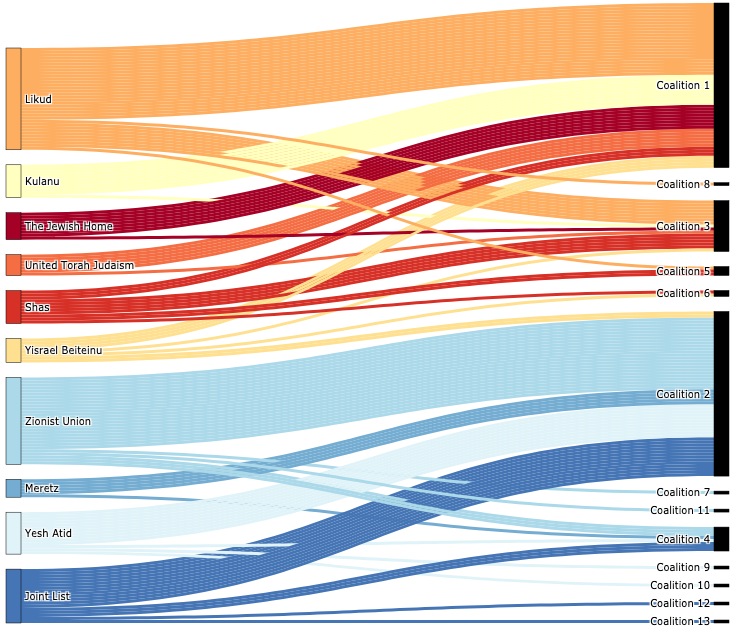
\includegraphics[width=\columnwidth]{pac_friends}
\caption{Coalitions formed by the PAC friends model, compared to party affiliations. Left wing parties are colored with blue hues, right wing red hues, center yellow hues.}
\end{figure}

\begin{table}[h!]
\centering
\begin{tabular}{c|c|c|c|c}
\hline
\multirow{2}{*}{ PAC Model } & \multicolumn{2}{c|}{ No. Coalitions } & \multicolumn{2}{|c}{ Norm Info Dist } \\
& mean & variance & mean & variance \\
\hline
Value Function & 87 & 0 & 0.526 & 0 \\
Friends & 13 & 1.6669 & 0.617 & 0.0003 \\
Selective friends & 20 & 3.3391 & 0.598 & 0.0001 \\
\hline
\end{tabular}
\caption{Each PAC model is implemented using the PAC top covering algorithm; choice set approximation are done with $3/4$ of all bills; the model is executed 50 times on the same Knesset dataset.}
\label{table:pac_models}
\end{table}

\bibliography{references}
\bibliographystyle{aaai}

\end{document}

